\section{Study 3: removing the tools' overhead}
\label{sec:tools}

\paragraph{Profiling.} On development parts only, we timed every stage inside the tool calls of a scripted policy that uses the CADFit tools. Sketch extraction spent \eExtractFitShare\% of its time (\eProfileParts{} development parts) fitting lines and arcs to every profile on the plane; a function-level profile of one development part attributed most of that to two routines: duplicate-point removal by an all-pairs loop, and a greedy segmenter that refits the whole run with an SVD each time it extends by one point. Revolve fitting rotated points one at a time in Python, and every executed check reloaded and rebuilt the target.

\paragraph{The revised package (tools v3).} Four changes are exact rewrites, each checked against the old code on development inputs: KD-tree duplicate removal (identical output on \eDedup{} randomized cases), the segment error from running sums with the old SVD fit deciding whenever a value lies within $10^{-6}$ (relative) of a threshold it is compared with (identical fitted output on \eFit{} sketches from \eFitParts{} development parts and 9 planes; fitting time \eFitOld\,s $\to$ \eFitNew\,s together with the first change), vectorized rotation (bit-identical on \eRotation{} cases), and loading the target once per process in the judge (\eJudge{} identical); the checks are recorded in \texttt{results/tools/equivalence.json}. One change alters behaviour: each executed check gets at most 120\,s. A step whose check does not finish stays in the model unchecked and is never delivered while a checked valid program exists. The study tests this package as a whole; it does not separate the rewrites from the cap.

\paragraph{Design.} The protocol fixed, before any run and before the cohort was drawn: tools \{v2, v3\} $\times$ toolset \{code, CADFit\} $\times$ \{Opus, Sonnet\} on the 40 fresh3 parts, three episodes each (960 episodes), same budget and settings as Study 2, each version running from its own frozen tree, delivered programs re-judged offline. The primary comparison is Opus with CADFit tools, v3 $-$ v2; the Opus family (primary, CADFit tools v3 $-$ code v3, code v3 $-$ v2) is Holm-corrected over three sign tests; the same comparisons for Sonnet are reported uncorrected. Runtime summaries were prespecified; timing contrasts and their tests are descriptive. Episodes lost to API credit exhaustion, rate limits, a faulty node and one client timeout crash were set aside and rerun before any analysis (\cref{app:log}).

\begin{figure}[t]
\centering
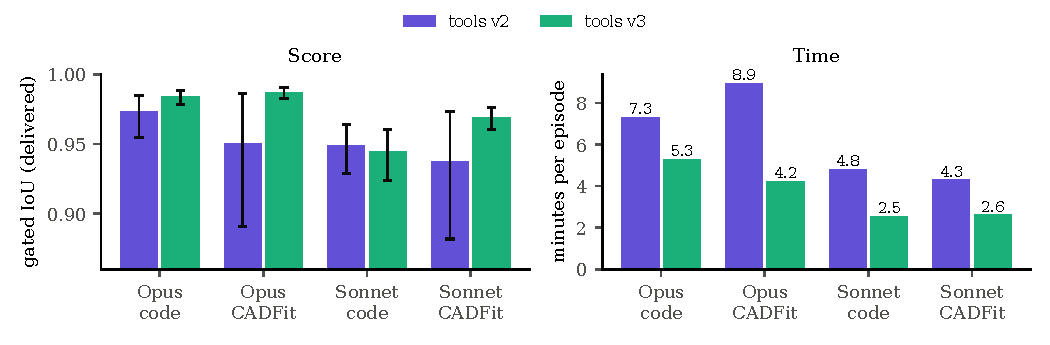
\includegraphics[width=\linewidth]{figures/tools_v3.pdf}
\caption{Study 3, 40 fresh3 parts, three episodes per part and condition. Left: gated IoU of the delivered program (95\% interval). Right: mean minutes per episode (means without intervals).}
\label{fig:tools}
\end{figure}

\begin{table}[t]
\centering
\small
\caption{Study 3 comparisons (gated IoU, paired over parts; better/worse at $\pm10^{-9}$; sign test $p$; Holm over the three Opus tests). Below: mean minutes per part, v3 $-$ v2 (descriptive), with parts faster.}
\label{tab:tools}
\setlength{\tabcolsep}{4pt}
\begin{tabular}{@{}llccc@{}}
\toprule
Comparison & & Difference \& 95\% interval & Better/worse & $p$ (Holm) \\
\midrule
Opus & CADFit v3 $-$ v2 (primary) & \tOpusSkillsVersion{} \tOpusSkillsVersionCI & \tOpusSkillsVersionWL & \tOpusSkillsVersionP{} (\tOpusSkillsVersionHolm) \\
Opus & CADFit v3 $-$ code v3 & \tOpusSkillsVsCode{} \tOpusSkillsVsCodeCI & \tOpusSkillsVsCodeWL & \tOpusSkillsVsCodeP{} (\tOpusSkillsVsCodeHolm) \\
Opus & code v3 $-$ v2 & \tOpusCodeVersion{} \tOpusCodeVersionCI & \tOpusCodeVersionWL & \tOpusCodeVersionP{} (\tOpusCodeVersionHolm) \\
Sonnet & CADFit v3 $-$ v2 & \tSonnetSkillsVersion{} \tSonnetSkillsVersionCI & \tSonnetSkillsVersionWL & \tSonnetSkillsVersionP \\
Sonnet & CADFit v3 $-$ code v3 & \tSonnetSkillsVsCode{} \tSonnetSkillsVsCodeCI & \tSonnetSkillsVsCodeWL & \tSonnetSkillsVsCodeP \\
Sonnet & code v3 $-$ v2 & \tSonnetCodeVersion{} \tSonnetCodeVersionCI & \tSonnetCodeVersionWL & \tSonnetCodeVersionP \\
\midrule
\multicolumn{2}{@{}l}{Minutes, v3 $-$ v2} & Opus CADFit \tTimeOpusSkills{} \tTimeOpusSkillsCI & faster on \tTimeOpusSkillsFaster/40 & \tTimeOpusSkillsP \\
 & & Opus code \tTimeOpusCode{} \tTimeOpusCodeCI & \tTimeOpusCodeFaster/40 & \tTimeOpusCodeP \\
 & & Sonnet CADFit \tTimeSonnetSkills{} \tTimeSonnetSkillsCI & \tTimeSonnetSkillsFaster/40 & \tTimeSonnetSkillsP \\
 & & Sonnet code \tTimeSonnetCode{} \tTimeSonnetCodeCI & \tTimeSonnetCodeFaster/40 & \tTimeSonnetCodeP \\
\bottomrule
\end{tabular}
\end{table}

\paragraph{Results.} The primary comparison is positive, \tOpusSkillsVersion{} \tOpusSkillsVersionCI, but its declared sign test does not establish an improvement ($p=\tOpusSkillsVersionP$, Holm \tOpusSkillsVersionHolm); we do not read it as evidence of no effect either (\cref{tab:tools}). With tools v3, Opus delivers a valid program in all \tOpusSkillsVThreeValid{} episodes with the CADFit tools (v2: \tOpusSkillsVTwoValid, with \tOpusSkillsVTwoNoOut{} no-output and \tOpusSkillsVTwoInvalid{} invalid), and those tools beat plain code by \tOpusSkillsVsCode{} \tOpusSkillsVsCodeCI, better on \tOpusSkillsVsCodeWL{} parts, Holm $p=\tOpusSkillsVsCodeHolm$: a small but consistent advantage, the reverse of the sign seen with tools v2 in Study 2. For Sonnet the same contrast is \tSonnetSkillsVsCode{} \tSonnetSkillsVsCodeCI{} (uncorrected $p=\tSonnetSkillsVsCodeP$). The best cell, Opus with CADFit tools v3, scores \tOpusSkillsVThree{} \tOpusSkillsVThreeCI. Across all 960 episodes, \tDeliveredValid{} delivered programs are valid offline, of which \tValidUnverified{} had not completed an in-episode check.

\paragraph{Time.} Mean minutes per part with the CADFit tools fall from \tOpusSkillsVTwoMin{} to \tOpusSkillsVThreeMin{} for Opus, faster on \tTimeOpusSkillsFaster{} of 40 parts, and from \tSonnetSkillsVTwoMin{} to \tSonnetSkillsVThreeMin{} for Sonnet. In the other cells the mean also falls, but the per-part sign tests are not significant, and the means are dominated by a few parts that used to run long. Opus with code v2 reproduces Study 2 on this new cohort (\tOpusCodeVTwo{} here, \cOpusCode{} there).
